% questions.tex —— 2010 年·普通高等学校招生考试·天津卷·文科 · 题目内容片段（无答案）
% 由 tools/generate_projects.py 依来源总账自 2010/2010_数学真题_天津文_试题.md 生成，勿手改（改源 MD 后重跑）


状态：needs-review；依固定候选 PDF 的勘误版两页（印刷页 637–638）逐题核验，六幅图已矢量重绘。原页未印分值，不补。第 3 题按上游勘误版题面转录（原固定件该页与该题自相矛盾）。

\gkpart{一、选择题}

\begin{question}
\gkti{1}$i$ 是虚数单位，复数 $\dfrac{3+i}{1-i}=$（　）

（A）$1+2i$

（B）$2+4i$

（C）$-1-2i$

（D）$2-i$

\end{question}
\begin{question}
\gkti{2}设变量 $x,y$ 满足约束条件 $\begin{cases}x+y\leqslant3,\\ x-y\geqslant-1,\\ y\geqslant1,\end{cases}$ 则目标函数 $z=4x+2y$ 的最大值为（　）

（A）$12$

（B）$10$

（C）$8$

（D）$2$

\Needspace{0.4\textheight}
\end{question}
\begin{question}
\gkti{3}阅读下面的程序框图，运行相应的程序，则输出 $s$ 的值为（　）
\nopagebreak[4]
\begin{center}% 2010 年天津卷文科第 3 题：程序框图，输出 s 的值。
% 来源 PDF：普通高考/2010/2010天津文.pdf（上游勘误版），SHA-256 e6b06813e17b7c332b651b8784c8fab0fcad0c8666ea6032a2958917c55307c9。
% 原页：第 1 页（A3 四栏）第 1 栏中部，书页码 637。
% 重绘依据：开始 → s=1 → i=1 → s=s(3−i)+1 → i=i+1 → 判断 i>4；
%   是（下）→ 输出 s → 结束；否（右）回到 s=s(3−i)+1 上方。
\begin{tikzpicture}[scale=0.66, semithick, >=Stealth,
  node distance=2.8mm, every node/.style={inner sep=2pt, font=\small}]
  \node (start) [draw, rounded corners=4pt, minimum width=1.7cm, minimum height=0.52cm] {开始};
  \node (init) [draw, minimum width=1.7cm, minimum height=0.52cm, below=of start] {$s=1$};
  \node (idx) [draw, minimum width=1.7cm, minimum height=0.52cm, below=of init] {$i=1$};
  \node (step) [draw, minimum width=4.3cm, minimum height=0.52cm, below=of idx] {$s=s\cdot(3-i)+1$};
  \node (inc) [draw, minimum width=1.9cm, minimum height=0.52cm, below=of step] {$i=i+1$};
  \node (cond) [draw, diamond, aspect=1.9, minimum width=2.2cm, minimum height=0.8cm, below=of inc] {$i>4?$};
  \node (out) [draw, trapezium, trapezium left angle=70, trapezium right angle=110,
    minimum width=2.2cm, minimum height=0.52cm, below=of cond] {输出 $s$};
  \node (end) [draw, rounded corners=4pt, minimum width=1.7cm, minimum height=0.52cm, below=of out] {结束};
  \draw[->] (start) -- (init);
  \draw[->] (init) -- (idx);
  \draw[->] (idx) -- (step);
  \draw[->] (step) -- (inc);
  \draw[->] (inc) -- (cond);
  \draw[->] (cond) -- (out);
  \node[anchor=west] at ($(cond.south)!0.5!(out.north)+(10pt,-2pt)$) {是};
  \draw[->] (cond.east) -- ++(0.8,0) |- node[pos=0.25, right] {否} (step.north);
  \draw[->] (out) -- (end);
\end{tikzpicture}
\end{center}
\nopagebreak[4]
（A）$-1$

（B）$0$

（C）$1$

（D）$3$

\end{question}
\begin{question}
\gkti{4}函数 $f(x)=\mathrm e^x+x-2$ 的零点所在的一个区间是（　）

（A）$(-2,-1)$

（B）$(-1,0)$

（C）$(0,1)$

（D）$(1,2)$

\end{question}
\begin{question}
\gkti{5}下列命题中，真命题是（　）

（A）$\exists m\in\mathbf R$，使函数 $f(x)=x^2+mx$（$x\in\mathbf R$）是偶函数

（B）$\exists m\in\mathbf R$，使函数 $f(x)=x^2+mx$（$x\in\mathbf R$）是奇函数

（C）$\forall m\in\mathbf R$，使函数 $f(x)=x^2+mx$（$x\in\mathbf R$）是偶函数

（D）$\forall m\in\mathbf R$，使函数 $f(x)=x^2+mx$（$x\in\mathbf R$）是奇函数

\end{question}
\begin{question}
\gkti{6}设 $a=\log_54$，$b=(\log_53)^2$，$c=\log_45$，则（　）

（A）$a<c<b$

（B）$b<c<a$

（C）$a<b<c$

（D）$b<a<c$

\end{question}
\begin{question}
\gkti{7}设集合 $A=\{x\mid|x-a|<1,x\in\mathbf R\}$，$B=\{x\mid1<x<5,x\in\mathbf R\}$。

若 $A\cap B=\varnothing$，则实数 $a$ 的取值范围是（　）

（A）$\{a\mid0\leqslant a\leqslant6\}$

（B）$\{a\mid a\leqslant2\text{ \text{或} }a\geqslant4\}$

（C）$\{a\mid a\leqslant0\text{ \text{或} }a\geqslant6\}$

（D）$\{a\mid2\leqslant a\leqslant4\}$

\Needspace{0.4\textheight}
\end{question}
\begingroup
\renewenvironment{question}{\Needspace{0.5\textheight}}{}
\begin{question}
\gkti{8}如图是函数 $y=A\sin(\omega x+\varphi)$（$x\in\mathbf R$）在区间 $\left[-\dfrac\pi6,\dfrac{5\pi}6\right]$ 上的图象，为了得到这个函数的图象，只要将 $y=\sin x$（$x\in\mathbf R$）的图象上所有的点（　）
\nopagebreak[4]
\begin{center}% 2010 年天津卷文科第 8 题：区间 [−π/6, 5π/6] 上的 y=A sin(ωx+φ) 图象。
% 来源 PDF：普通高考/2010/2010天津文.pdf（上游勘误版），SHA-256 e6b06813e17b7c332b651b8784c8fab0fcad0c8666ea6032a2958917c55307c9。
% 原页：第 1 页（A3 四栏）第 2 栏上部，书页码 637。
% 重绘依据：曲线过 (−π/6,0)、(π/3,0)、(5π/6,0)，在 π/12 取最大值 1，在 7π/12 取最小值 −1。
\begin{tikzpicture}[semithick, x=2.4cm, y=1.5cm, every node/.style={inner sep=1.2pt, font=\small}]
  \draw[-stealth] (-0.62,0) -- (3.0,0) node[below] {$x$};
  \draw[-stealth] (0,-1.35) -- (0,1.45) node[left] {$y$};
  \node[below left] at (0,0) {$O$};
  \draw[thick,domain=-0.5236:2.6180,samples=160] plot (\x,{sin(2*\x r + pi/3 r)});
  \draw[dashed] (0,-1) -- (1.5,-1);
  \draw (-0.5236,0.04) -- (-0.5236,-0.04) node[below left] {$-\dfrac\pi6$};
  \draw (1.0472,0.04) -- (1.0472,-0.04) node[below] {$\dfrac\pi3$};
  \draw (2.6180,0.04) -- (2.6180,-0.04) node[below] {$\dfrac{5\pi}6$};
  \draw (-0.04,1) -- (0.04,1) node[left] {$1$};
  \draw (-0.04,-1) -- (0.04,-1) node[left] {$-1$};
\end{tikzpicture}
\end{center}
\nopagebreak[4]
（A）向左平移 $\dfrac\pi3$ 个单位长度，再把所得各点的横坐标缩短到原来的 $\dfrac12$ 倍，纵坐标不变

（B）向左平移 $\dfrac\pi3$ 个单位长度，再把所得各点的横坐标伸长到原来的 $2$ 倍，纵坐标不变

（C）向左平移 $\dfrac\pi6$ 个单位长度，再把所得各点的横坐标缩短到原来的 $\dfrac12$ 倍，纵坐标不变

（D）向左平移 $\dfrac\pi6$ 个单位长度，再把所得各点的横坐标伸长到原来的 $2$ 倍，纵坐标不变

\Needspace{0.4\textheight}
\end{question}
\endgroup
\begin{question}
\gkti{9}如图，在 $\triangle ABC$ 中，$AD\perp AB$，$\overrightarrow{BC}=\sqrt3\overrightarrow{BD}$，$|\overrightarrow{AD}|=1$，则 $\overrightarrow{AC}\cdot\overrightarrow{AD}=$（　）
\nopagebreak[4]
\begin{center}% 2010 年天津卷文科第 9 题：三角形 ABC 中 AD⊥AB，D 在 BC 上。
% 来源 PDF：普通高考/2010/2010天津文.pdf（上游勘误版），SHA-256 e6b06813e17b7c332b651b8784c8fab0fcad0c8666ea6032a2958917c55307c9。
% 原页：第 1 页（A3 四栏）第 2 栏中部，书页码 637。
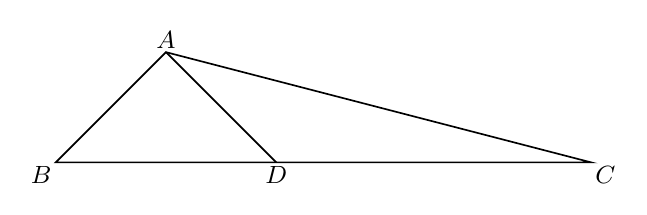
\begin{tikzpicture}[semithick, every node/.style={inner sep=1.2pt, font=\small}]
  \coordinate (A) at (-1.2,1.4);
  \coordinate (B) at (-2.6,0);
  \coordinate (D) at (0.2,0);
  \coordinate (C) at (4.2,0);
  \draw (A) -- (B) -- (C) -- cycle;
  \draw (A) -- (D);
  \node[above] at (A) {$A$};
  \node[below left] at (B) {$B$};
  \node[below] at (D) {$D$};
  \node[below right] at (C) {$C$};
\end{tikzpicture}
\end{center}
\nopagebreak[4]
（A）$2\sqrt3$

（B）$\dfrac{\sqrt3}2$

（C）$\dfrac{\sqrt3}3$

（D）$\sqrt3$

\end{question}
\begin{question}
\gkti{10}设函数 $g(x)=x^2-2$（$x\in\mathbf R$），

\nopagebreak[4]
\[f(x)=\begin{cases}g(x)+x+4,&x<g(x),\\ g(x)-x,&x\geqslant g(x).\end{cases}\]

则 $f(x)$ 的值域是（　）

（A）$\left[-\dfrac94,0\right]\cup(1,+\infty)$

（B）$[0,+\infty)$

（C）$\left[-\dfrac94,+\infty\right)$

（D）$\left[-\dfrac94,0\right]\cup(2,+\infty)$

\end{question}
\gkpart{二、填空题}

\Needspace{0.4\textheight}
\begin{question}
\gkti{11}如图，四边形 $ABCD$ 是圆 $O$ 的内接四边形，延长 $AB$ 和 $DC$ 相交于点 $P$。若 $PB=1$，$PD=3$。

则 $\dfrac{BC}{AD}$ 的值为$\underline{\qquad}$。
\nopagebreak[4]
\begin{center}% 2010 年天津卷文科第 11 题：圆内接四边形 ABCD，AB 与 DC 延长交于 P。
% 来源 PDF：普通高考/2010/2010天津文.pdf（上游勘误版），SHA-256 e6b06813e17b7c332b651b8784c8fab0fcad0c8666ea6032a2958917c55307c9。
% 原页：第 1 页（A3 四栏）第 2 栏下部，书页码 637。
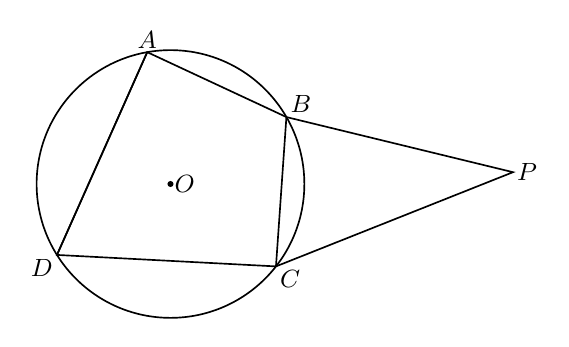
\begin{tikzpicture}[semithick, every node/.style={inner sep=1.2pt, font=\small}]
  \coordinate (O) at (0,0);
  \coordinate (A) at (100:1.7);
  \coordinate (B) at (30:1.7);
  \coordinate (C) at (-38:1.7);
  \coordinate (D) at (212:1.7);
  \coordinate (P) at (4.35,0.15);
  \draw (O) circle (1.7);
  \fill (O) circle (1.1pt);
  \node[right] at (O) {$O$};
  \draw (A) -- (B) -- (P) -- (C) -- (D) -- cycle;
  \draw (B) -- (C);
  \draw (A) -- (D);
  \node[above] at (A) {$A$};
  \node[above right] at (B) {$B$};
  \node[below right] at (C) {$C$};
  \node[below left] at (D) {$D$};
  \node[right] at (P) {$P$};
\end{tikzpicture}
\end{center}
\nopagebreak[4]
\Needspace{0.4\textheight}
\end{question}
\begingroup
\renewenvironment{question}{\Needspace{0.5\textheight}}{}
\begin{question}
\gkti{12}一个几何体的三视图如图所示，则这个几何体的体积为$\underline{\qquad}$。
\nopagebreak[4]
\begin{center}% 2010 年天津卷文科第 12 题：正视图、侧视图与俯视图。
% 来源 PDF：普通高考/2010/2010天津文.pdf（上游勘误版），SHA-256 e6b06813e17b7c332b651b8784c8fab0fcad0c8666ea6032a2958917c55307c9。
% 原页：第 1 页（A3 四栏）第 3 栏上部，书页码 637。
% 重绘依据：正视图为 2×1 矩形、中分；侧视图为 1×1 矩形；俯视图为梯形，上底 2、下底 1、高 2。
\begin{tikzpicture}[semithick, every node/.style={inner sep=1.2pt, font=\small}]
  % 正视图
  \draw (0,4.2) rectangle (2,5.2);
  \draw (1,4.2) -- (1,5.2);
  \node[below] at (1,3.7) {正视图};
  \draw[<->] (0,5.45) -- (1,5.45) node[midway,above] {$1$};
  \draw[<->] (1,5.45) -- (2,5.45) node[midway,above] {$1$};
  \draw[<->] (-0.4,4.2) -- (-0.4,5.2) node[midway,left] {$1$};
  % 侧视图
  \draw (3.4,4.2) rectangle (4.4,5.2);
  \node[below] at (3.9,3.7) {侧视图};
  \draw[<->] (3.4,5.45) -- (4.4,5.45) node[midway,above] {$1$};
  % 俯视图
  \draw (0,0) -- (1,0) -- (2,2) -- (0,2) -- cycle;
  \draw[<->] (0,-0.35) -- (1,-0.35) node[midway,below] {$1$};
  \draw[<->] (-0.4,0) -- (-0.4,2) node[midway,left] {$2$};
  \node[below] at (1.1,-0.95) {俯视图};
\end{tikzpicture}
\end{center}
\nopagebreak[4]
\end{question}
\endgroup
\begin{question}
\gkti{13}已知双曲线 $\dfrac{x^2}{a^2}-\dfrac{y^2}{b^2}=1$（$a>0$，$b>0$）的一条渐近线方程是 $y=\sqrt3x$，它的一个焦点与抛物线 $y^2=16x$ 的焦点相同。则双曲线的方程为$\underline{\qquad}$。

\end{question}
\begin{question}
\gkti{14}已知圆 $C$ 的圆心是直线 $x-y+1=0$ 与 $x$ 轴的交点，且圆 $C$ 与直线 $x+y+3=0$ 相切。

则圆 $C$ 的方程为$\underline{\qquad}$。

\end{question}
\begin{question}
\gkti{15}设 $\{a_n\}$ 是等比数列，公比 $q=\sqrt2$，$S_n$ 为 $\{a_n\}$ 的前 $n$ 项和。记 $T_n=\dfrac{17S_n-S_{2n}}{a_{n+1}}$，$n\in\mathbf N^*$。设 $T_{n_0}$ 为数列 $\{T_n\}$ 的最大项，则 $n_0=$ $\underline{\qquad}$。

\end{question}
\begin{question}
\gkti{16}设函数 $f(x)=x-\dfrac1x$，对任意 $x\in[1,+\infty)$，$f(mx)+mf(x)<0$ 恒成立，则实数 $m$ 的取值范围是$\underline{\qquad}$。

\end{question}
\gkpart{三、解答题}

\begin{question}
\gkti{17}在 $\triangle ABC$ 中，$\dfrac{AC}{AB}=\dfrac{\cos B}{\cos C}$。

（1）证明：$B=C$；

（2）若 $\cos A=-\dfrac13$，求 $\sin\left(4B+\dfrac\pi3\right)$ 的值。

\end{question}
\begin{question}
\gkti{18}有编号为 $A_1,A_2,\cdots,A_{10}$ 的 $10$ 个零件，测量其直径（单位：$\mathrm{cm}$），得到下面数据：

\begin{center}
\begingroup\setlength{\tabcolsep}{4pt}
\begin{tabular}{lllllllllll}
\toprule
编号 & $A_1$ & $A_2$ & $A_3$ & $A_4$ & $A_5$ & $A_6$ & $A_7$ & $A_8$ & $A_9$ & $A_{10}$ \\
\midrule
直径 & $1.51$ & $1.49$ & $1.49$ & $1.51$ & $1.49$ & $1.51$ & $1.47$ & $1.46$ & $1.53$ & $1.47$ \\
\bottomrule
\end{tabular}
\endgroup
\end{center}

其中直径在区间 $[1.48,1.52]$ 内的零件为一等品。

（1）从上述 $10$ 个零件中，随机抽取一个，求这个零件为一等品的概率；

（2）从一等品零件中，随机抽取 $2$ 个。

① 用零件的编号列出所有可能的抽取结果；

② 求这 $2$ 个零件直径相等的概率。

\Needspace{0.4\textheight}
\end{question}
\begingroup
\renewenvironment{question}{\Needspace{0.5\textheight}}{}
\begin{question}
\gkti{19}如图，在五面体 $ABCDEF$ 中，四边形 $ADEF$ 是正方形，$FA\perp$ 平面 $ABCD$，$BC\parallel AD$，$CD=1$，$AD=2\sqrt2$，$\angle BAD=\angle CDA=45^\circ$。

（1）求异面直线 $CE$ 与 $AF$ 所成角的余弦值；

（2）证明 $CD\perp$ 平面 $ABF$；

（3）求二面角 $B-EF-A$ 的正切值。
\nopagebreak[4]
\begin{center}% 2010 年天津卷文科第 19 题：五面体 ABCDEF。
% 来源 PDF：普通高考/2010/2010天津文.pdf（上游勘误版），SHA-256 e6b06813e17b7c332b651b8784c8fab0fcad0c8666ea6032a2958917c55307c9。
% 原页：第 2 页（A3 四栏）第 1 栏下部，书页码 638。
% 重绘依据：ADEF 为正方形，FA⊥平面 ABCD；底面 ABCD 中 BC∥AD。
% 可见棱实线，FA 与 AD 两条被遮挡的棱画虚线。
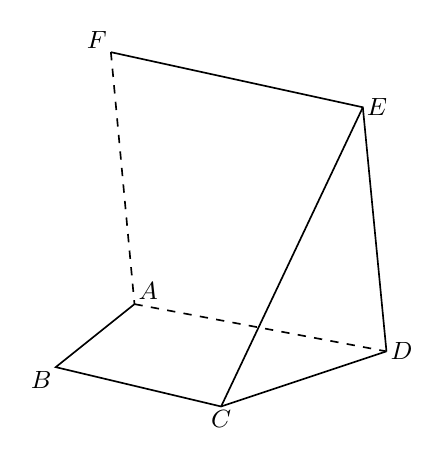
\begin{tikzpicture}[semithick, every node/.style={inner sep=1.2pt, font=\small}]
  \coordinate (F) at (0.2,4.4);
  \coordinate (E) at (3.4,3.7);
  \coordinate (A) at (0.5,1.2);
  \coordinate (D) at (3.7,0.6);
  \coordinate (B) at (-0.5,0.4);
  \coordinate (C) at (1.6,-0.1);
  \draw (F) -- (E) -- (D);
  \draw[dashed] (F) -- (A);
  \draw (A) -- (B) -- (C) -- (D);
  \draw[dashed] (A) -- (D);
  \draw (C) -- (E);
  \node[above left] at (F) {$F$};
  \node[right] at (E) {$E$};
  \node[above right] at (A) {$A$};
  \node[right] at (D) {$D$};
  \node[below left] at (B) {$B$};
  \node[below] at (C) {$C$};
\end{tikzpicture}
\end{center}
\nopagebreak[4]
\end{question}
\endgroup
\begin{question}
\gkti{20}已知函数 $f(x)=ax^3-\dfrac32x^2+1$（$x\in\mathbf R$），其中 $a>0$。

（1）若 $a=1$，求曲线 $y=f(x)$ 在点 $(2,f(2))$ 处的切线方程；

（2）若在区间 $\left[-\dfrac12,\dfrac12\right]$ 上，$f(x)>0$ 恒成立，求 $a$ 的取值范围。

\end{question}
\begin{question}
\gkti{21}已知椭圆 $\dfrac{x^2}{a^2}+\dfrac{y^2}{b^2}=1$（$a>b>0$）的离心率 $e=\dfrac{\sqrt3}2$，连接椭圆的四个顶点得到的菱形的面积为 $4$。

（1）求椭圆的方程；

（2）设直线 $l$ 与椭圆相交于不同的两点 $A$、$B$，已知点 $A$ 的坐标为 $(-a,0)$。

① 若 $|AB|=\dfrac{4\sqrt2}5$，求直线 $l$ 的倾斜角；

② 若点 $Q(0,y_0)$ 在线段 $AB$ 的垂直平分线上，且 $\overrightarrow{QA}\cdot\overrightarrow{QB}=4$，求 $y_0$ 的值。

\end{question}
\begin{question}
\gkti{22}在数列 $\{a_n\}$ 中，$a_1=0$，且对任意 $k\in\mathbf N^*$，$a_{2k-1}$，$a_{2k}$，$a_{2k+1}$ 成等差数列，其公差为 $2k$。

（1）证明 $a_4$，$a_5$，$a_6$ 成等比数列；

（2）求数列 $\{a_n\}$ 的通项公式；

（3）记 $T_n=\dfrac{2^2}{a_2}+\dfrac{3^2}{a_3}+\cdots+\dfrac{n^2}{a_n}$，证明 $\dfrac32<2n-T_n\leqslant2$（$n\geqslant2$）。

\end{question}